\documentclass{scrbook}

\usepackage[dvipsnames,table]{xcolor}
\usepackage{amsmath, amssymb, amsfonts, amsthm}
\usepackage{mathtools}
\usepackage{cancel}
\usepackage[ngerman]{babel}
\usepackage{enumerate}
\usepackage{framed}
\usepackage{hyperref}
\usepackage[utf8]{inputenc}
\usepackage[a4paper,left=2cm,right=2cm,top=1.5cm,bottom=1cm,includeheadfoot]{geometry}
\usepackage{graphicx}
\usepackage[amssymb]{SIunits}
\usepackage{tikz}
\usepackage{tikz-3dplot}
\usepackage{ulem}
\usepackage{wasysym}

\setlength{\parindent}{0cm}
\makeatletter
\@addtoreset{chapter}{part}
\makeatother
\usepackage{etoolbox}
\makeatletter
\patchcmd{\chapter}{\if@openright\cleardoublepage\else\clearpage\fi}{}{}{}
\makeatother

\theoremstyle{remark}
\newtheorem*{goal}{Ziel}

\theoremstyle{plain}
\newtheorem*{theorem}{Satz}

\theoremstyle{definition}
\newtheorem{definition}{Definition}[section]

\tdplotsetmaincoords{60}{110}

\usetikzlibrary{3d, arrows, decorations, trees}

\newcommand{\Pl}{{\mathrm{Pl}}}
\newcommand{\parsec}{{\mathrm{pc}}}
\newcommand{\AU}{{\mathrm{AU}}}

\title{Skript - Einführung in die Astronomie und Astrophysik}
\author{Transkribiert von\\ Martine Lenders}

\begin{document}
\maketitle

\tableofcontents

\part{Klassische Astronomie}
\chapter{Koordinatensysteme, Zeit, Sternörter}
\section{Grundlagen der sphärischen Astronomie}
\subsection{Bezugssysteme}
\begin{itemize}
    \item Orientierung: Konstellationen am Himmel\\
        $\rightarrow$ \textbf{Problem:} systematische Bewegung\\
        $\Rightarrow$ \textbf{Bezugssystem mit Fixpunkten}
    \item Symmetrie $\mapsto$ Kuppelkoordinaten \\
        $\hookrightarrow$ Fixierung an Drehimpulsvektoren
    \item Koordinatenursprung im Schwerpunkt
\end{itemize}

\subsection{Äquatorialsystem}
\begin{goal}
    Positionsbeschreibung im Inertialsystem, Fixierung an Drehimpulsvektoren
    der Erdbewegung
\end{goal}

\begin{description}
    \item[Eigendrehimpuls]  $\vec n_e$
    \item[Bahndrehimpuls]   $\vec n_b$
    \item[Einheitsvektor in Richtung Frühlingspunkt]   $\vec n_{\vernal}$
\end{description}

\begin{equation}
    (\vec n_e \times \vec n_b) = \vec n_{\vernal}
\end{equation}

\begin{definition}
    Orthonormalsystem Äquatorialsystem: $(\vec n_e$, $\vec n_{\vernal}$, $(\vec n_e \times \vec n_{\vernal}))$
\end{definition}

\begin{center}
    \begin{tikzpicture}[scale=4,tdplot_main_coords]
        \pgfmathsetmacro{\rvec}{0.8}
        \pgfmathsetmacro{\alphavec}{60}
        \pgfmathsetmacro{\deltavec}{30}

        \coordinate (O) at (0,0,0);
        \tdplotsetcoord{S}{\rvec}{\deltavec}{\alphavec}

        \draw [->, thick] (O) -- (1, 0, 0) node[anchor=north east] {$\vec n_{\vernal}$};
        \draw [->, thick] (O) -- (0, 1, 0) node[anchor=north west] {$(\vec n_e \times \vec n_{\vernal})$};
        \draw [->, thick] (O) -- (0, 0, 1) node[anchor=south] {$\vec n_e$};

        \tdplotsetrotatedcoords{60}{40}{30}

        \tdplotdrawarc[dashed]{(O)}{1.5}{0}{360}{anchor=south west}{Himmelsäquator}
        \draw [->] (O) -- (S) node [pos=0.5, anchor=south east] {$r$};
        \draw [dotted] (O) -- (Sxy);
        \draw [dotted] (Sxy) -- (S) node [anchor=south west] {$\vec n$};
        \tdplotdrawarc[dotted]{(O)}{0.3}{0}{\alphavec}{anchor=south}{$\alpha$}
        \tdplotsetthetaplanecoords{\alphavec}
        \tdplotdrawarc[dotted, tdplot_rotated_coords]{(O)}{0.2}{\deltavec}{90}{anchor=east}{$\delta$}
    \end{tikzpicture}
    \[ \vec n = \sin \delta \cdot \vec n_e + \cos \delta \cdot \cos \alpha \cdot \vec n_{\vernal} + \cos \delta \cdot \sin \alpha \cdot (\vec n_e \times \vec n_{\vernal}) \]
\end{center}

\begin{itemize}
    \item $\alpha$: Rektaszension [$^\mathrm{h}$, $^\mathrm{m}$, $^\second$]
    \item $\delta$: Deklination [$\degree$, $\arcminute$, $\arcsecond$]
    \item Umrechnung: $360\degree \mathrel{\hat=} 24^\mathrm{h} \Leftrightarrow 15\degree \mathrel{\hat=} 1^\mathrm{h}$
    \item \textbf{Position eines astronomischen Objektes}: $\boxed{(\alpha, \delta)\text{-Angabe}}$
    \item Koordinaten Frühlingspunkt: $(0, 0)$
\end{itemize}

\subsection[Horizontsystem]{Horizontsystem (lokales irdisches Koordinatensystem)}
\begin{description}
    \item[Zenitvektor] $\vec n_z$, Richtung: Erdmittelpunkt -- Beobartungsposition
         Erdoberfläche
     \item[Nadir] Fußpunkt
     \item[Horizontebene]
         \begin{itemize}
             \item Vektor in Nordrichung: $\vec n_N$
             \item Vektor in Westrichtung: $\vec n_W = \vec n_z \times \vec n_N$
         \end{itemize}
     \item[Azimut] $\varphi$
     \item[Höhe] $h$
     \item[Zenitdistanz] $z = 90\degree - h \Leftrightarrow z + h = 90\degree$
\end{description}

\begin{definition}
    Ortonormalsystem Horizontsystem: $(\vec n_z, \vec n_N, \vec n_W)$
\end{definition}


\begin{center}
    \begin{tikzpicture}[scale=4,tdplot_main_coords]
        \pgfmathsetmacro{\rvec}{0.8}
        \pgfmathsetmacro{\phivec}{120}
        \pgfmathsetmacro{\hvec}{30}

        \coordinate (O) at (0,0,0);
        \tdplotsetcoord{S}{\rvec}{\hvec}{\phivec}

        \draw [->, thick] (O) -- (1, 0, 0) node[anchor=north east] {$\vec n_N$};
        \draw [->, thick] (O) -- (0, 1, 0) node[anchor=north west] {$\vec n_W$};
        \draw [->, thick] (O) -- (0, 0, 1) node[anchor=south] {$\vec n_z$};

        \tdplotsetrotatedcoords{60}{40}{30}

        \tdplotdrawarc[dashed]{(O)}{1.5}{0}{360}{anchor=south west}{Horizontebene}
        \draw [->] (O) -- (S) node [pos=0.5, anchor=south east] {$r$};
        \draw [dotted] (O) -- (Sxy);
        \draw [dotted] (Sxy) -- (S) node [anchor=south west] {$\vec n$};
        \tdplotdrawarc[dotted]{(O)}{0.3}{0}{\phivec}{anchor=south east}{$\varphi$}
        \tdplotsetthetaplanecoords{\phivec}
        \tdplotdrawarc[dotted, tdplot_rotated_coords]{(O)}{0.2}{\hvec}{90}{anchor=30}{$h$}
        \tdplotdrawarc[<-, dotted, tdplot_rotated_coords]{(O)}{0.2}{0}{\hvec}{anchor=70}{$z$}
    \end{tikzpicture}

    \textbf{Position}: $(\varphi, z)$ oder $(\varphi, h)$
    \[ \vec n = \sin \delta \cdot \vec n_W + \cos \delta \cdot \cos \alpha \cdot \vec n_N + \cos \delta \cdot \sin \alpha \cdot \vec n_z \]
\end{center}

\begin{description}
    \item[wahrer Horizont] Ebene durch Erdmittelpunkt
    \item[schwere Nachteile]
        \begin{itemize}
            \item Koordinaten sind ortsabhängig
            \item Koordinaten sind zeitabhängig
        \end{itemize}
\end{description}

\subsection[Globale irdische Koordinaten]{Globale irdische Koordinaten $(l, b)$}
\begin{goal}
    Position des Beobachters $\vec n_z$ global angeben
\end{goal}
\begin{center}
    \begin{tikzpicture}[scale=4,tdplot_main_coords]
        \pgfmathsetmacro{\rvec}{0.8}
        \pgfmathsetmacro{\lvec}{100}
        \pgfmathsetmacro{\bvec}{16}

        \coordinate (O) at (0,0,0);
        \tdplotsetcoord{S}{\rvec}{\bvec}{\lvec}
        \tdplotsetcoord{G}{1.5}{51.5}{0}

        \draw [->, thick] (O) -- (1, 0, 0) node[anchor=north east] {$\vec n_1$};
        \draw [->, thick] (O) -- (0, 1, 0) node[anchor=north west] {$\vec n_2$};
        \draw [->, thick] (O) -- (0, 0, 1) node[anchor=south] {$\vec n_e$};

        \tdplotsetrotatedcoords{60}{40}{30}

        \tdplotdrawarc[dashed]{(O)}{1.5}{0}{360}{anchor=south west}{Äquator}
        \draw [->] (O) -- (S) node [pos=0.5, anchor=south east] {$r$};
        \draw [->] (O) -- (G) node [anchor=south east] {$\vec n_z^G$};
        \draw [dotted] (O) -- (Sxy);
        \draw [dotted] (Sxy) -- (S) node [anchor=south west] {$\vec n_z$};
        \tdplotdrawarc[dotted]{(O)}{0.21}{0}{\lvec}{anchor=south east}{$l$}
        \tdplotsetthetaplanecoords{\lvec}
        \tdplotdrawarc[dotted, tdplot_rotated_coords]{(O)}{0.2}{\bvec}{90}{anchor=30}{$b$}
        \tdplotsetthetaplanecoords{0}
        \tdplotdrawarc[dashed, tdplot_rotated_coords]{(O)}{1.5}{90}{-90}{anchor=east}{Nullmeridian}
    \end{tikzpicture}
    \[ \vec n_z = \sin \delta \cdot \vec n_e + \cos \delta \cdot \cos \alpha \cdot \vec n_1 + \cos \delta \cdot \sin \alpha \cdot \vec n_2 \]
\end{center}
$\hookrightarrow$ 1. Nachteil: Ausgleich der Ortsabhängigkeit

\subsection{Beziehung zwischen den Koordinatensystemen}
\subsubsection{Projektion auf Himmelsäquator}
\begin{description}
    \item[Winkel $\Theta$] von Projektion von $\vec n_z$ bei $\vec n_{\vernal}$ \\
        $\rightarrow$ Sternzeit $[ \mathrm{h} : \mathrm{m} : \second ]$
    \item[Speziell] $\Theta_G$ Sternzeit Greenwich
        \[ \underbrace{\Theta(l)}_{\vec n_z} = \underbrace{\Theta_G}_{\vec n_z^G} - l \]
    \item[Sternzeit $\rightarrow$ Uhrzeit] Beispiel: $\Theta_G$
        \begin{align*}
            \Theta_G(t) &= \underbrace{\Theta_G(0)}_{t = 0\,\mathrm{h}} + t\left(\frac{367.24}{365.24}\right) \\
            1\,\mathrm{a} &= \underbrace{366.24\,\mathrm{d}}_{\text{Sterntage}} = \underbrace{365.24\,\mathrm{d}}_{\text{normale Tage}} \\
                          &\Rightarrow \text{1 Sterntag ist kürzer als ein normaler Tag}
        \end{align*}
\end{description}

\begin{itemize}
    \item $\tau$: Winkel zwischen projezierten $\vec n_z$ und projezierten $\vec n$ (Objekt) \\
        $\rightarrow$ Stundenwinkel\\
        $\Rightarrow$ Sternzeit ist der Stundenwinkel des Frühlingspunkts
    \item Beziehung zwischen den Koordinatensystemen:
        \[ \boxed{\tau = \Theta(l, t) - \alpha = \theta_G(0) + t \left(\frac{366.24}{365.24}\right) - l - \alpha} \]
        $\rightarrow$ Beobachtung: $(\tau, \delta)$
\end{itemize}

\subsection{Ekliptikales System}
\begin{description}
    \item[ekliptikale Länge] $\lambda$
    \item[ekliptikale Breite] $\beta$
\end{description}
\[ \varepsilon = 23\degree 27\arcsecond \]

\begin{center}
    \begin{tikzpicture}[scale=4,tdplot_main_coords]
        \pgfmathsetmacro{\rvec}{0.8}
        \pgfmathsetmacro{\lvec}{80}
        \pgfmathsetmacro{\bvec}{20}

        \coordinate (O) at (0,0,0);
        \tdplotsetcoord{S}{\rvec}{\bvec}{\lvec}
        \tdplotsetcoord{n_e}{1.5}{23.4}{0}

        \draw [->, thick] (O) -- (1, 0, 0) node[anchor=north east] {$\vec n_{\vernal}$};
        \draw [->, thick] (O) -- (0, 1, 0) node[anchor=north west] {$(\vec n_b \times \vec n_{\vernal})$};
        \draw [->, thick] (O) -- (0, 0, 1) node[anchor=south] {$\vec n_b$};

        \tdplotsetrotatedcoords{60}{40}{30}

        \tdplotdrawarc[dashed]{(O)}{1.5}{0}{360}{anchor=south west}{Äquator}
        \draw [->] (O) -- (S);
        \draw [->] (O) -- (n_e) node [anchor=south east] {$\vec n_e$};
        \draw [dotted] (O) -- (Sxy);
        \draw [dotted] (Sxy) -- (S);
        \tdplotdrawarc[dotted]{(O)}{0.21}{0}{\lvec}{anchor=south east}{$\lambda$}
        \tdplotsetthetaplanecoords{\lvec}
        \tdplotdrawarc[dotted, tdplot_rotated_coords]{(O)}{0.2}{\bvec}{90}{anchor=30}{$\beta$}
        \tdplotsetthetaplanecoords{0}
        \tdplotdrawarc[dashed, tdplot_rotated_coords]{(O)}{0.5}{0}{23.4}{anchor=north}{$\varepsilon$}
    \end{tikzpicture}
    \[ \vec n_z = \sin \delta \cdot \vec n_e + \cos \delta \cdot \cos \alpha \cdot \vec n_1 + \cos \delta \cdot \sin \alpha \cdot \vec n_2 \]
\end{center}

\subsection{Galaktische Koordinaten}
\begin{center}
    \begin{tikzpicture}[scale=4,tdplot_main_coords]
        \pgfmathsetmacro{\rvec}{0.8}
        \pgfmathsetmacro{\lvec}{115}
        \pgfmathsetmacro{\bvec}{70}

        \coordinate (O) at (0,0,0);
        \coordinate (GZ) at (0,1,0);
        \tdplotsetcoord{S}{\rvec}{\bvec}{\lvec}
        \tdplotsetcoord{n_e}{1.5}{23.4}{0}

        \tdplotsetrotatedcoords{60}{40}{30}

        \tdplotdrawarc{(GZ)}{1.5}{0}{360}{anchor=south west}{}
        \node at (O) {$\astrosun$};
        \draw [thick] (O) -- (GZ);
        \node at (GZ) {$\circ$};
        \node [anchor=west] at (GZ) {$GZ$};
        \node [anchor=north] at (GZ) {Sagitarius A$^*$};
        \draw [->] (O) -- (S) node {$\star$};
        \draw [->] (GZ) -- (0,1,1);
        \draw [dotted] (O) -- (Sxy);
        \draw [dotted] (Sxy) -- (S);
        \tdplotdrawarc[dotted]{(O)}{0.7}{90}{\lvec}{anchor=east}{$l$}
        \tdplotsetthetaplanecoords{\lvec}
        \tdplotdrawarc[dotted, tdplot_rotated_coords]{(O)}{0.6}{\bvec}{90}{anchor=30}{$b$}
    \end{tikzpicture}
\end{center}

\paragraph{Galaktisches Zentrum (GZ)}
\begin{align*}
    \alpha &= 17^\mathrm{h}42^\mathrm{m}25^\second \\
    \delta &= -28\degree 55\arcminute
\end{align*}

\section{Bahnen der Himmelskörper im Horizontsystem}
\begin{center}
    \framebox{Erddrehung $\Rightarrow$ tägliche Bewegung}
\end{center}
\paragraph{Ausgezeichnete Punkte}
\begin{itemize}
    \item Aufgang und Untergang:
        \begin{itemize}
            \item Parallelkreis-Horizont
            \item Schnittpunkt
        \end{itemize}
    \item obere Kulmination: $h_1 = 90\degree - |b - \delta|$
    \item untere Kulmination: $h_1 = -90\degree + |b + \delta|$
\end{itemize}

\paragraph{Speziell}
\begin{itemize}
    \item Zirkumpolare Sterne: $\delta > 90\degree - |b|$
    \item nie sichtbar: $\delta < -90\degree + |b|$
\end{itemize}

\paragraph{Änderung der Höhe mit der Zeit}
\[ h(t) = \arcsin(\sin b \sin \delta + \cos b \cos \delta \cos \tau) \]

\paragraph{Näherung} ($h$ klein)
\[ h \approx \delta + (90\degree - b) \cos \tau \]

\section{Komplikationen: Veränderungen der Koordinaten}
\paragraph{Ursache} Drehimpuls \emph{nicht} raumfest
\paragraph{wichtigste Störungen}
\begin{itemize}
    \item lunisolare Präzession
    \item Nutation
    \item Planetenpräzession
\end{itemize}

\subsection{Lunisolare Präzession}
\[
    \left.
    \begin{array}{lr@{\ }l}
        \text{Äquatorradius:} & a &= 6378.14\,\kilo\metre \\
        \text{Polradius:} & b &= 6346.755\,\kilo\metre
    \end{array}
    \right\} \Delta \approx 21.4 \kilo\metre
\]

Abplattung der Erde:
\[ \varphi = \left(\frac{a - b}{a}\right) = \frac{1}{298.253} \]
$\Rightarrow$ \framebox{Kreisel}

Präzession im Kraftfeld: Mond --  Sonne

\begin{center}
    \begin{tikzpicture}[scale=3,tdplot_main_coords]

        \coordinate (O) at (0,0,0);
        \tdplotsetcoord{S}{1}{23.5}{-90}

        \draw [gray,thick] (1, -2.2, 0) -- (1, 2.2, 0) node [right] {\color{black} Ekliptik};
        \draw [gray,dotted] (0.5, -2.2, 0) -- (0.5, 2.2, 0);
        \draw [gray,thick] (0, -2.2, 0) -- (0, 2.2, 0);
        \draw [gray,dotted] (-0.5, -2.2, 0) -- (-0.5, 2.2, 0);
        \draw [gray,thick] (-1, -2.2, 0) -- (-1, 2.2, 0);

        \draw [gray,thick] (1.5, -2, 0) -- (-1.5, -2, 0);
        \draw [gray,dotted] (1.5, -1.5, 0) -- (-1.5, -1.5, 0);
        \draw [gray,thick] (1.5, -1, 0) -- (-1.5, -1, 0);
        \draw [gray,dotted] (1.5, -0.5, 0) -- (-1.5, -0.5, 0);
        \draw [gray,thick] (1.5, 0, 0) -- (-1.5, 0, 0);
        \draw [gray,dotted] (1.5, 0.5, 0) -- (-1.5, 0.5, 0);
        \draw [gray,thick] (1.5, 1, 0) -- (-1.5, 1, 0);
        \draw [gray,dotted] (1.5, 1.5, 0) -- (-1.5, 1.5, 0);
        \draw [gray,thick] (1.5, 2, 0) -- (-1.5, 2, 0);

        \draw (0,-2.1,0) -- (0, 2.2, 0) node[anchor=west] {Äquator};
        \draw (0,1.7,0.678) -- (0,-1.7,-0.678);
        \draw [->] (O) -- (0, 0, 1) node[anchor=south] {$\vec n_b$};
        \draw [->] (O) -- (S) node[anchor=south] {$\vec n_e$};

        \tdplotdrawarc[->]{(Sz)}{0.3987}{0}{360}{}{}
        \tdplotsetthetaplanecoords{90}
        \tdplotdrawarc[dotted, tdplot_rotated_coords]{(O)}{1}{90}{66.5}{anchor=east}{$\sim 23.5\degree$}
        \tdplotsetthetaplanecoords{-90}
        \tdplotdrawarc[dotted, tdplot_rotated_coords]{(O)}{0.5}{23.5}{0}{anchor=north}{$\sim 23.5\degree$}
    \end{tikzpicture}
\end{center}

\paragraph{Folge} 
Erdrotationsachse $\vec n_e$ rotiert in $\sim 25700$ Jahren um den Pol der
Ekliptik $\vec n_b$

\subsection{Nutation}
\paragraph{Problem} Mondbahn ist gegen die Ekliptik um $5.15\degree$ geneigt\\
$\Rightarrow$ Präzession: 18.6 Jahre

\subsection{Planetenpräzession}
Einfluss der Planeten auf die Erdbahn\\
$\Rightarrow$ Verschiebung des Frühlingspunkts um $\sim 0.1\arcsecond$ pro Jahr \\
$\hookrightarrow$ Problem: Zeitabhängigkeit

\section{Sternörter}
\begin{itemize}
    \item \textbf{Sternbild:} IAU 1928 feste Grenzen für Sternbilder: 88 Sternbilder
    \item \textbf{Sternnamen:}\\
        Problem: mehrdeutig / kompliziert
        \begin{itemize}
            \item 78 hellsten Sterne mit historischen Namen\\
                z. B. Sirius, Wega, Aldebaran, Algol, ...
            \item seit 1603 (\textsc{Beyer}): kleine griechische Buchstaben + 
                Genitiv des lateinischen Sternbildnamen\\
                z. B. $\alpha$ Ori, $\gamma$ UMa, $\varepsilon$ Cyg

                Sequenz: meist Helligkeit, manchmal Konstellation im Sternbild
            \item \textsc{Flamsteed:} Buchstaben $\rightarrow$ Nummern in 
                Reihenfolge der Rektaszension im Sternbild\\
                z. B. 22, 20, 23, 21 Her

                \textbf{Problem:} Reihenfolge nicht stabil!
            \item \textbf{Moderne Bezeichnung:} \framebox{Katalog + Katalognummer}\\
                z. B. HD 483705 (meist Rektanzension, HD = \textsc{Henry} -- \textsc{Draper})
            \item \textbf{Folge:} Vielfachbezeichnung\\
                z. B. Wega = $\alpha$ Lyr = 3 Lyr = HR7001 = DM383230 = SAO 67174
            \item speziell: Doppelsterne

                \textbf{Index:} Puchstaben / Ziffern \\
                z. B. Sirius A, Begleiter: Sirius B
            \item Variable Sterne
            \item Röntgenquellen / Radioquellen
        \end{itemize}
    \item Datenbank: SIMBAD
\end{itemize}

\section{Bezugssysteme der Zeit}
\begin{itemize}
    \item Fixpunkte der Zeitrechnung $\rightarrow$ bevorzugte Positionen bezüglich
        der rotierenden Bezugussysteme
    \item Maßeinheiten der Zeit: Periodizität\\
        Tag, Jahr
\end{itemize}

\paragraph{ursprünglich} Sonne $\longrightarrow$ Tag
\paragraph{wahre Sonnenzeit} Stundenwinkel der Sonne (obere Kulmination $\longrightarrow$ obere Kulmination) \\
$\rightarrow$ angezeigt durch Sonnenuhr
\paragraph{Problem} ungleichmäßig $\Rightarrow$ praktisch unbrauchbar
\paragraph{Ursachen}
\begin{enumerate}
    \item Ellipsenbahnen $\Rightarrow$ 2. \textsc{Kepler}'sches Gesetz
    \item Projektionseffekt
\end{enumerate}

\paragraph{Lösung} Definition einer mittleren Sonnenzein mit gleicher
    Geschwindigkeit auf dem Äquator\\
    $\Rightarrow$ mittlere Sonnenzeit
\paragraph{Differenz} Zeitgleichung
\[ \boxed{z = \text{wahre Sonnenzeit} - \text{mittlere Sonnenzeit}} \]
\[ z(t) = -0.27^{\mathrm{m}} + 7.18^{\mathrm{m}} \sin(\underbrace{\omega t + 178\degree}_{\text{Ellipse}}) +
          9.85^{\mathrm{m}} \sin(\underbrace{2 \omega t + 201\degree}_{\text{Projektion}}), \qquad
      \omega = \frac{360\degree}{267.2422\,\mathrm{d}}\]

\begin{itemize}
    \item UT: universal time -- Einheit: mittlerer Sonnentag (Greenwich)
    \item GMST: mittlere Sternzeit in Greenwich
    \item TAI: internationale Atomzeit -- Einheit: $\second$
\end{itemize}

\paragraph{Kalender} Problem: Bezugspunkt für Jahreslänge $\Rightarrow$
    unterschiedliche "`Jahre"'

\paragraph{Jahr} kein ganzes Vielfaches eines Tages\\
$\Rightarrow$ Schaltjahre und Kalenderreformen

\paragraph{Lösung} Astronomen vewenden das Julianische Datum
\[ \text{JD}\underbracket{\text{xxxxx}}_{\text{Tage}}.\underbracket[1pt][1.2em]{\text{xx}}_{\mathclap{\text{Stunden, Minuten, Sekunden}}} \qquad \text{gemessen \emph{nur} in Tagen} \]

\chapter{Himmelsmechanik}
\section{Kinematik}
\subsection*{vor Newton}
\begin{description}
    \item[Aufgabe] genaue Beschreibung der scheinbaren Bewengung
        \begin{itemize}
            \item \emph{nicht} die Erklärung/das Verständnis des zugrunde
                  liegenden Sachverhaltes (Gesetztes)
        \end{itemize}
    \item[speziell] scheinbare Planetenbahnen $\rightarrow$ Mars
        \begin{center}
            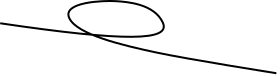
\includegraphics[width=.3\textwidth]{img/ptolemaeus_mars.pdf}
        \end{center}
    \item[Modelle]
        \begin{itemize}
            \item \textsc{Ptolemäus:}
                \begin{itemize}
                    \item Geozentrisch (Erde im Zentrum)
                    \item Planeten auf Epizykelbahnen
                \end{itemize}
            \item \textsc{Kopernikus:}
                \begin{itemize}
                    \item Heliozentrisch (Sonne im Zentrum)
                    \item \emph{Kreisbahnen}
                \end{itemize}
        \end{itemize}
    \item[Enscheidung] z. B. Planetenphasen der inneren Planeten\\
        $\Rightarrow$ Kopernisches Weltbild
\end{description}
\begin{itemize}
    \item \textsc{Kepler:} Messung d. Marsbahnen (T. \textsc{Brahe})\\
          $\Rightarrow$ \textsc{Kepler}'sche Gesetze (empirisch)
          \begin{enumerate}
              \item Ellipsen, Sonne in einem Brennpunkt
              \item Flächensatz $\Leftrightarrow$ Drehimpulserhaltung \\
                    Radiusvektoren überstreichen in gleicher Zeit gleiche Flächen,\\
                    d. h. Flächengeschwindigkeit = $\mathbf{const}$
              \item Umlaufzeiten/Abstände ($a$: Halbachse, $T$: Umlaufzeit)
                      \[ \frac{a^3}{T^2} \sim \mathbf{const} \]
          \end{enumerate}
\end{itemize}

\section{Newton'sche Mechanik}
\textsc{Newton}'sche Axiome:
\begin{enumerate}[(i)]
    \item Trägheitsgesetz (Masse konstant, vergl. spezielle Relativitätstheorie):
        \[ \vec p = m \vec v = m \dot{\vec{r}} = m \frac{d}{dt} \vec r \]
    \item Impulsänderung durch Krafteinwirkung:
        \[ \frac{d}{dt} \vec p = \dot{\vec p} = \vec F = m \ddot{\vec r} = m \frac{d^2}{dt^2} \vec r = m \vec a \]
    \item Actio = Reactio:
        \[ \vec F_{ik} = -\vec F_{ki} \]
\end{enumerate}

\section{2-Körperproblem -- Kepler Gesetze}
\paragraph{Skizze:}
\begin{center}
    \tdplotsetrotatedcoords{0}{0}{90}
    \begin{tikzpicture}[scale=2,tdplot_rotated_coords]
        \coordinate (O) at (0,0,0);
        \coordinate [label=left:{$m_1$}] (m1) at (-1,1,-0.2);
        \coordinate [label=right:{$m_2$}] (m2) at (1,1.2,0.4);
        \coordinate (S) at (0,1.1,0.1);

        \draw [thick,->] (O) -- (1.2,0,0) node [anchor=north west] {$x$};
        \draw [thick,->] (O) -- (0,1.2,0) node [anchor=south west] {$y$};
        \draw [thick,->] (O) -- (0,0,1.2) node [anchor=south] {$z$};

        \draw [->] (O) -- (m1) node [pos=0.5,anchor=north east] {$\vec r_1$};
        \draw [->] (O) -- (m2) node [pos=0.5,anchor=north west] {$\vec r_2$};
        \draw [->] (m1) -- (m2) node [pos=0.5, anchor=south] {$\vec r$};
        \draw [->] (O) -- (S) node [pos=0.5, anchor=east] {$R$};
    \end{tikzpicture}
\end{center}

\paragraph{DGL}
\begin{align*}
    m_1 \vec r_1 + m_2 \vec r_2 = \frac{d^2}{dt^2} (m_1 \vec r_1 + m_2 \vec r_2) &= \vec 0 \tag*{$| \dfrac{m}{m}$} \\
    \Rightarrow m \frac{d^2}{dt^2} \underbrace{\left(\frac{m_1\vec r_1 + m_2 \vec r_2}{m}\right)}_{\mathclap{= \vec R = \frac{\vec C_2}{m} \text{für $\vec C_1 = \vec P_{\mathrm{ges}}$}}} = \vec 0 \Leftrightarrow m \ddot{\vec{R}} &= \vec 0
\end{align*}
\[ \boxed{m\ddot{\vec{R}} = \vec 0} \]
\framebox{$\Rightarrow$ Referezsystem bzgl. Massenschwerpunkt muss ein Inertialsystem sein}

$\Rightarrow$ \textbf{Wahl:} Koordinatenursprung im Schwerpunkt $\Leftrightarrow \vec{R} = \vec 0$

\section{Bemerkungen zu Störeffekten}
\paragraph{Problem} $N$-Körperproblem nicht allgemein lösbar!

\paragraph{Methode}
\begin{itemize}
    \item Ansatz einenr Störungstheorie
    \item numerische Behandlung des $N$-Körperproblems
    \item \sout{statistische Methoden}
\end{itemize}

\paragraph{Aller einfachster Ansatz}
\textbf{Situation:}
\begin{center}
    \begin{tikzpicture}
        \coordinate (M) at (0, 0);
        \node [above] at (M) {$\mathcal{M}$};
        \coordinate (m) at (2, 0);
        \node [above] at (m) {$m$};
        \coordinate (mS) at (5, 0);
        \node [above] at (mS) {$m_S$};
        \filldraw(M) circle (1pt);
        \filldraw(m) circle (1pt);
        \filldraw(mS) circle (1pt);

        \draw (M) -- (m) node [pos=0.5, above] {$a$};
        \draw (m) -- (mS) node [pos=0.5, above] {$d$};
        \draw [->, >=stealth'] (6,1) node [right] {störende Masse} -- (5.5,0.5);
    \end{tikzpicture}
\end{center}

\paragraph{Anmerkung} kleine Störung

\paragraph{Abschätzung} maximaler Einfluss (Konjunktion / Opposition)

\paragraph{Beschleunigungen}
\[ b_m = \frac{G m_S}{d^2}; \qquad b_{\mathcal{M}} = \frac{G m_S}{(a + d)^2} \]

$\Rightarrow$ Störbeschleunigung: $\Delta b = b_m - b_{\mathcal M} = G m_S (\frac{1}{d^2} - \frac{1}{(d + a)^2})$

$a \ll d$: Reihenentwicklung
\[ \boxed{\text{Taylorentwicklung:} f(x) = f(x_0) + f'(x_0) \cdot (x - x_0) + \dots} \]

\begin{align*}
    \frac{1}{x^2} &\approx \frac{1}{x_0^2} - \frac{2}{x_0^3} (x - x_0) + 0, \text{mit} x = a + d; x_0 = d \\
    \Rightarrow \frac{1}{(a+d)^2} &= \frac{1}{d^2} - \frac{2}{d^3} (a + \cancel{d} - \cancel{d}) + 0 \\
    \Rightarrow a b &= \frac{Gm_S 2 a}{d^3} = \frac{2 G \mathcal{M}}{a^2} \cdot f
\end{align*}

\begin{definition}
    Störfaktor $f$: \[ \boxed{f := \frac{m_S}{\mathcal{M}} \cdot \left(\frac{a}{d}\right)^3} \]
\end{definition}

je größer $f$ $\Rightarrow$ wichtiger Einfluss auf Bahnen
\begin{center}
\begin{tabular}{ll}
    Erde $\xrightarrow{\text{durch}}$ Venus: & $f \approx \dfrac{1}{37000}$ \\
    Erde $\xrightarrow{\text{durch}}$ Jupiter: & $f \approx \dfrac{1}{53000}$ \\
    Erde $\xrightarrow{\text{durch}}$ Saturn: & $f \approx \dfrac{1}{360}$
\end{tabular}
\end{center}

$\rightarrow$ Numerische Simulation: $N$-body simulation

\section{Virialsatz}
\begin{framed}
    \begin{theorem}
        Die Gesamtenergie $E$ eines gravitativ gebundenen Systems $(E < 0)$ im 
        Gleichgewicht ist immer gleich der Hälfte der zeitgemittelten potentiellen
        Energie $\langle E_{\mathrm{pot}} \rangle$ des Systems:
        \[ E = \frac{\langle E_{\mathrm{pot}} \rangle}{2} \Leftrightarrow \langle E_{\mathrm{kin}} \rangle = - \frac{\langle E_{\mathrm{pot}} \rangle}{2}\]
    \end{theorem}
\end{framed}

\paragraph{Betrachte}
\begin{align*}
    Q &\underset{\mathclap{
        \begin{array}{c}
            \uparrow \\
            \text{Summe über alle Teilchen $i$ des Systems}
        \end{array}
        }}{=} \sum\limits_{i} \langle\vec p_i, \vec r_i\rangle = \sum\limits_{i} m_i \frac{d}{dt} \langle\vec r_i, \vec r_i\rangle\\
        \Rightarrow \frac{dQ}{dt} &= \sum\limits_{i} (\langle\dot{\vec{p}}_i, \vec r\rangle + \langle\vec p, \dot{\vec{r}}_i\rangle)
        = \frac{d}{dt} \sum\limits_i m_i \underbrace{\langle\dot{\vec{r}}_i, \vec{r}_i\rangle}_{= ?}
\end{align*}

\color{OliveGreen}
\textbf{Nebenrechnung:}
\begin{align*}
    \frac{d}{dt} \langle\vec{r}_i, \vec{r}_i\rangle &= 2 \langle\vec{r}_i, \dot{\vec{r}}_i\rangle = \frac{d}{dt} (r_i)^2 \\
    \Rightarrow \langle\vec{r}_i, \dot{\vec{r}}_i\rangle &= \frac{1}{2} \frac{d}{dt} r_i^2 \\
\color{black}
\Rightarrow \dot Q &\color{black}=\frac{d}{dt} \sum_i \frac{1}{2} \frac{d}{dt} (m_i r_i^2) = \frac{1}{2} \frac{d^2}{dt^2} \underbrace{\sum\limits_i (m_i r_i^2)}_{FI}
\end{align*}
\color{black}
$I$: Trägheitsmement der Teilchen des Systems
\begin{align*}
    \Rightarrow \dot Q &= \frac{1}{2} \ddot I    \tag*{$| - \sum\limits_i \langle \vec p_i, \dot{\vec{r}}_i\rangle$} \\
    \Rightarrow \frac{1}{2}\ddot I - \sum\limits_i \langle \vec p_i, \dot{\vec{r}}_i\rangle &= \sum\limits_i \langle \dot{\vec{p}}_i, \vec{r}_i\rangle = \underbrace{\sum\limits_i \langle\vec F_i \cdot \vec r_i\rangle}_{\text{\textsc{Clausius}' Virial}} \\
    \Rightarrow \frac{1}{2}\ddot I - \underbrace{\sum\limits_i m_i \langle \dot{\vec{r_i}}, \dot{\vec{r}}_i\rangle}_{= 2 E_{\mathrm{kin}}} &= \sum\limits_i \langle \vec{F}_i, \vec{r}_i\rangle \\
\end{align*}

$F_i$: Summe aller auf Teilchen $i$ wirkenden Kräfte

\paragraph{Betrachte} Gravitativ gebundenes System bestehend aus vielen Teilen

Es gilt:
\begin{align*}
    \sum\limits_i \langle\vec F_i, \vec r_i\rangle &= \sum\limits_i \left\langle\sum\limits_{j \neq i} \vec F_{ij}, \underbrace{\vec r_i}_{\mathclap{\qquad\qquad= \frac{1}{2} (\vec r_i - \vec r_j) + \frac{1}{2} (\vec r_i + \vec r_j)}}\right\rangle\\
                &= \frac{1}{2} \sum\limits_i \left\langle\sum\limits_{j \neq i} \vec F_{ij}, \underbrace{\vec r_i - \vec r_j}_{=: - \vec r_{ij}}\right\rangle + \underbrace{\frac{1}{2} \sum\limits_i \left\langle\sum\limits_{j \neq i} \vec F_{ij}, \vec r_i + \vec r_j\right\rangle}_{= 0; \vec F_{ij} = -\vec F_{ji}} \\
    \vec F_{ij} &= \left(\frac{Gm_im_j}{r_{ij}^2}\right) \cdot \vec r_{ij} \tag{Gravitationskraft $i \Leftrightarrow j$}\\
    \Rightarrow \sum\limits_i \langle\vec F_i, \vec r_i\rangle &= -\frac{1}{2} \sum\limits_i\left(\sum\limits_{j \neq i} \left(\frac{Gm_im_j}{r_{ij}^{\cancel{3}}}\right) \underbrace{\langle\vec r_{ij}, \vec r_{ij}\rangle}_{= \cancel{r_{ij}^2}}\right)\\
        &= -\frac{1}{2} \sum\limits_i \left(\sum\limits_{j \neq i} \frac{G m_i m_j}{r_{ij}}\right) = \frac{1}{2} \sum\limits_i \sum\limits_{j \neq i} E_{\mathrm{pot}_{ij}} = E_{\mathrm{pot}}\\
    \underset{=0}{\cancel{\frac{1}{2} \langle\ddot I\rangle}} - 2 \langle E_{\mathrm{kin}} &= \langle E_{\mathrm{pot}}\rangle
\end{align*}

\paragraph{Zeitmittlung} \[\langle \cdot \rangle = \frac{1}{2} \int\limits_0 \cdot\ dt\]

\color{OliveGreen}
\textbf{Nebenrechnung:}
\begin{itemize}
    \item $\langle \ddot I \rangle = \frac{1}{2} \int\limits_0^{\tau} \ddot I\ dt = \dot I |_0^{\tau} = \underbrace{\dot I(\tau) - \dot I(0)}_{=0}$ (periodische Orbit-Mittlung über eine Periode)
    \item System im Gleichgewicht: $I = \mathbf{const} \Rightarrow \dot I = 0$
\end{itemize}
\color{black}


\begin{align*}
    \Rightarrow \langle E_{\mathrm{pot}}\rangle &= -2 \langle E_{\mathrm{kin}} \rangle \\
    \text{oder}\qquad \langle E\rangle &= \langle E_{\mathrm{pot}} \rangle + \langle E_{\mathrm{kin}} \rangle = 
    \langle E_{\mathrm{pot}} \rangle - \frac{1}{2} \langle E_{\mathrm{pot}} \rangle = \frac{\langle E_{\mathrm{pot}} \rangle}{2}
\end{align*}

\paragraph{Anwendung des Virialsatzes}
\begin{itemize}
    \item ideales Gas
    \item Kugelsternhaufen
    \item Galaxiehaufen
    \item Sternentstehung
    \item Himmelsmechanik
    \item ...
\end{itemize}

\part{Planeten}
\chapter{Physikalische Eigenschaften des Sonnensystems}
\section{Stabilität der Atmosphäre}
\paragraph{Frage} Warum cerliert ein Planet seine Atmosphäre?
\paragraph{Einfache Abschätzung} Energiegleichgewicht
\[ E_{\mathrm{kin}} = E_{\mathrm{grav}} \]
$\Rightarrow$ Entweichgeswindigkeit eines Teilchens mit der Masse $m$ an der 
              Planetenoberfläche
\[ \frac{\cancel{m}}{2} v_{\mathrm{esc}}^2 = \frac{G \cancel{m} m_{\mathrm{Pl}}}{R_{\mathrm{Pl}}} \]

\[ \Rightarrow v_{\mathrm{esc}} = \sqrt{\frac{2 G m_{\mathrm{Pl}}}{R_{\mathrm{Pl}}}} \]

Geschwindigkeitsverteilungsfunktion eines Gases
\[ f(\vec v)\ dv^3: \int f (\vec v)\ dv^3 = 1 \tag{Normierung} \]

z. B. \textbf{\textsc{Maxwell}-Geschwindigkeitsverteilung}
\[ f(\vec v) = \left(\frac{m}{2 \pi T}\right)^{\frac{3}{2}} e^{-\frac{mv^2}{2} \per (k T)} \]

\[ \Rightarrow \frac{m v_{\mathrm{th}}^2}{2} \approx kT \Rightarrow \text{Thermische Geschwindigkeit $v_{\mathrm{th}} = \sqrt{\dfrac{2 k T}{m}}$}\]

\paragraph{Bruchteil der entweichenden Teilchen $\delta$}
\begin{align*}
    \delta &:= \int\limits_{\mathclap{\vec k \cdot \vec v > v_{\mathrm{esc}}}} f(\vec v)\ dv^3 \tag{$\vec k$: Normalvektor der Atmosphäre}
\end{align*}

\paragraph{Vorteil} $v_{\mathrm{esc}}$ klein: $m_{\mathrm{Pl}}$ klein, $R_{\mathrm{Pl}}$ groß \\
    $f(\vec v)$ groß: $T$ groß

\begin{definition}
    Stabilitätsparameter
    \[ \Gamma^2 := \left(\frac{v_{\mathrm{th}}}{v_{\mathrm{esc}}}\right)^2 = \left(\frac{kTR_{\mathrm{Pl}}}{G m_{\mathrm{Pl}} m}\right) \]
    \begin{tabular}{r@{:\ }l}
        $\Gamma \gg 1$ & instabil \\
        $\Gamma \ll 1$ & stabil
    \end{tabular}
\end{definition}

\paragraph{Planetenatmosphäre} (Thermischer Verlust) \\
$\Gamma$-Reihenfolge: Jupiter $>$ Saturn $>$ Neptun $>$ Uranus $>$ Erde $>$
Venus $>$ Mars $>$ Pluto $>$ Triton $>$ \emph{Titan} $>$ Io $>$ ... $>$ \emph{Merkur}
$>$ \emph{Mond} $>$ ...

\section{Energiehaushalt und Atmosphärentemperatur}
\paragraph{Anmerkung} Strahlungsgleichgewicht, Schwarzkörper
\[ \boxed{\text{Abstrahlung} = \underset{\begin{matrix}\Uparrow\\\text{Sonne}\end{matrix}}{\text{Einstrahlung}}} \]
 
\subsubsection{Energieabstrahlung der Sonne}
\[ L_{\astrosun} = \underbrace{4 \pi R_{\astrosun}^2}_{\text{Oberfläche}} \cdot \underset{\begin{matrix}\text{Strahlungsfluss}\\\text{[Energie / Zeit / Fläche]}\end{matrix}}{F_{\astrosun} (R_{\astrosun})} \leftarrow \text{Leuchtkraft der Sonne [Energie / Zeit]} \]

\begin{center}
    \begin{tikzpicture}[tdplot_main_coords]
        \tdplotdrawarc[dashed]{(0,0,0)}{2}{90}{270}{}{};
        \draw [->] (0,0,0) -- (0,2,0) node [above, pos=0.5] {$R_{\astrosun}$};
        \shade[ball color=red!10!yellow, opacity=0.50] (0,0,0) circle (2cm);
        \draw (0,0,0) circle (2cm);

        \tdplotdrawarc{(0,0,0)}{2}{-90}{90}{}{};
    \end{tikzpicture}
\end{center}

Schwarzkörper:
\[ B_{\nu}(T) \xrightarrow{\int\ d\nu} \boxed{F_{\astrosun} = \sigma T^4} \tag{Stefan-Boltzmann-Gesetz} \]
$\sigma$: Stefan-Boltzmann-Gesetz
\[ E_{\mathrm{ph}} = h\nu \]

\begin{center}
    \begin{tikzpicture}
        \draw (0,0) -- (7.4,0);

        \draw [domain=-90:90] plot ({cos(\x)}, {sin(\x)});
        \draw [domain=-41.81:41.81] plot ({3*cos(\x)}, {3*sin(\x)});
        \draw [domain=-16.6:16.6] plot ({7*cos(\x)}, {7*sin(\x)});
        \node (r) at (7,0) [anchor=south west] {$r$};
        \draw [->] (0,0) -- (41:1) node [pos=0.5] {$R_{\astrosun}$};
    \end{tikzpicture}
\end{center}

\paragraph{Energieerhaltung}
\begin{align*}
    L_{\astrosun} &= \cancel{4 \pi} R_{\astrosun}^2 F_{\astrosun} = \cancel{4 \pi} r^2 \boxed{f_{\astrosun}(r)}\\
f_{\astrosun}(r) &= F_{\astrosun} (R_{\astrosun}) \cdot \underbrace{\left(\frac{R_{\astrosun}}{r}\right)^2}_{\mathclap{\text{geometrische Verdünnung}}} \tag{Am Ort $r$ ankommender Strahlungsfluss}\\
    f_{\astrosun}(1\,\mathrm{AU}) &= 1.37\,\kilo\watt\metre^{-2} \tag{Solarkonstante}
\end{align*}

\paragraph{Absorbierte Energie}
\begin{align*}
L_{\mathrm{abs}} &= f_{\astrosun}(r) \cdot \underset{\mathclap{\begin{matrix}\uparrow\\\text{absorbierende Fläche}\end{matrix}}}{\mathcal{F}_{\mathrm{abs}}} \cdot (1 - A) + \underbrace{4 \pi R_{\mathrm{Pl}} f_Q}_{\mathclap{\text{innere Energiequelle}}}\\
    \text{Albedo $A$:}\ A &= \frac{\text{gestreutes / reflektiertes Licht}}{\text{einfallendes Licht}}
\end{align*}

\paragraph{Emittierte Energie}
\begin{align*}
L_{\mathrm{em}} &= f_{\mathrm{em}} \cdot \mathcal{F}_{\mathrm{em}} = \underbrace{\sigma \cdot T_{\mathrm{Pl}}^4}_{\mathclap{\begin{matrix}\downarrow\\\text{Abstrahlung erfolgt in $\mathbb{R}$}\end{matrix}}}\cdot \mathcal{F}_{\mathrm{em}} \cdot e^{- \tau_{\mathrm{IR}}}
\end{align*}
$\tau_{\mathrm{IR}}$: optische Tiefe

Gegeben: $L_{\mathrm{em}} = L_{\mathrm{abs}}$
\[ \cancel{\sigma} \cdot \left(\frac{R_{\astrosun}}{r}\right)^2 \cdot T_{\astrosun}^4 \cdot \mathcal{F}_{\mathrm{abs}} \cdot (1-A) + 4 \pi R_{\mathrm{Pl}} f_Q = \cancel{\sigma} \cdot T_{\mathrm{Pl}}^4 \cdot \mathcal{F}_{\mathrm{E}} \cdot e^{\tau_{IR}} \]

Gesucht: Strahlungsgleichgewichtstemperatur des Planeten ($f_Q = 0, \tau_{IR} = 0$)
\[ \boxed{T_{\mathrm{Pl}^2} = (1 - A) \left(\frac{\mathcal{F}_{\mathrm{abs}}}{\mathcal{F}_{\mathrm{em}}}\right) \left(\frac{R_{\astrosun}}{r}\right)^2 T_{\astrosun}^4} \]

Annahme:
\begin{align*}
    \mathcal F_{\mathrm{abs}} &= \pi R_{\mathrm{Pl}}^2 \\
    \mathcal F_{\mathrm{em}} &= \begin{cases}
        4 \pi R_{\mathrm{Pl}}^2, & \text{schnelle Rotation} \\
        2 \pi R_{\mathrm{Pl}}^2, & \text{langsame Rotation}
    \end{cases}
\end{align*}

Beispiel: Erde $A \approx 0.3$, $f_Q \approx 0.06 \watt\metre^{-2} \approx 10^{-4} f_{\astrosun}$
\begin{align*}
    r &= 1\,\mathrm{AU} & R_{\astrosun} &= 696000\,\kilo\metre & \\
    L_{\astrosun} &= 3.85 \cdot 10^{26}\,\watt & T_{\astrosun} &= 5780\,\kelvin
\end{align*}
\[ \Rightarrow T = \sqrt{3.787 \cdot 10^{-6}}\,T_{\astrosun} \approx 0.044\,T_{\astrosun} \approx 255\,\kelvin \]

\paragraph{Folgerung} tatsächliche Planetentemperatur $T_{\mathrm{Pl}}$ größer
als Strahlungsgleichgewichtstemperatur $T$
\[ \Rightarrow \boxed{T_{\mathrm{Pl}} = T} \]

\section{Stabilität eines Mondes (Planeten) gegenüber Störungen durch 
         Gezeitenkräfte}

\section{Bedingungen für Planetenentstehung}

\chapter{Extrasolare Planeten}
\section{Beobachtungsmethoden}
\begin{itemize}
    \item Alle Methoden wurden für Doppelsterne entwickelt!\\
        $\hookrightarrow$ "`neu"' größere Messgenauigkeit
\end{itemize}

\begin{center}
    \begin{tikzpicture}[
        edge from parent/.style = {->,draw},
        basic/.style = {text width=4cm, align=center},
        root/.style = {basic},
        level 1/.style = {sibling distance=8cm},
        level 2/.style = {basic, draw, rectangle, text width=5cm, sibling distance=3cm},
        level 3/.style = {basic, text width=3cm},
        >=latex]
        \node[root] {Messmethode}
            child {node [level 2] {dynamische Effekte}
                child {node [level 3] {
                        Ra"-dial"-ge"-schwind"-ig"-keits"-mess"-ung\\\framebox{RV-method}
                    }}
                    child {node [level 3] {
                        \framebox{Astrometrie}
                    }}
                }
            child {node [level 2] (photo) {photometrische Effekte}
                child {node [level 3] {Transit-methode}}
                child {node [level 3] {Mi"-cro"-lensing-Me"-tho"-de}}
                child {node [level 3] {Direkte\\Beobachtung}}
            };
    \end{tikzpicture}
\end{center}

\subsection{Radialgeschwindigkeitsmethode}
\paragraph{Prinzip} Messung der Radialgeschwindigkeit $v_r$ (in Sehstrahlrichtung)
aus hochaufgelösten Spektren über dem Doppler-Effekt

\begin{definition}
    Klassischer Doppler-Effekt
    \[ \boxed{\frac{v_r}{c} = \frac{\delta \lambda}{\lambda_0} = \frac{\lambda_{\text{beob}} - \lambda_0}{\lambda_0}} \]
\end{definition}

$\Rightarrow$ Radialgeschwindigkeitskurve $v_r(t)$

\begin{center}
    \begin{minipage}[h]{.25\textwidth}
        \centering
        \begin{tikzpicture}
            \draw [domain=60:120] plot ({0.2*cos(\x)}, {0.2*sin(\x)});
            \draw (120:.3) -- (0,0) -- (60:.3);
            \draw [thin] (0,0.5) -- (0,3.5);
            \draw (0,2.5) arc (-90:0:0.5);
            \node at (0.25,2.75) {$\cdot$};
            \draw [dashed, blue, ->] (0,3) -- (2,3) node [above, pos=0.5] {$\vec v_t$};
            \draw [thick, red, ->] (0,1) -- (0,3) node [left, pos=0.5] {$\vec v_r$};
            \draw [thick, ->] (0,1) -- (2,3) node [anchor=north west, pos=0.5] {$\vec v$};
        \end{tikzpicture}
    \end{minipage}
    \begin{minipage}[h]{.7\textwidth}
        \centering
        \begin{tikzpicture}[domain=0:7]
            \draw [<->] (0,-1) -- (0,2.0) node [anchor=south east] {$v_r [\metre\per\second]$};
            \draw [->] (0,0) -- (7,0) node [right] {$t [\second]$};
            \draw [dashed] (0,0.83) -- (7,0.83);
            \draw [samples=200,smooth] plot function{sin(3*x)+0.83};
            \draw [|<->|] (-0.1,0) -- (-0.1,0.83) node [left, pos=0.5] {$v_*$};
        \end{tikzpicture}
    \end{minipage}
\end{center}

\paragraph{Form} Bahnexzentrizität ($\varepsilon = 0$ $\Leftrightarrow$ Sinus-Formi) \\
$\hookrightarrow$ Exopleneten größere $\varepsilon$

\begin{itemize}
    \item Bestimmung der Bahnparameter durch Messung \emph{mehrerer} (!) Perioden
\end{itemize}

\paragraph{Problem}
\begin{itemize}
    \item Bestimmung der Planetenmasse \emph{nicht} möglich, sondern nur 
        $\boxed{m_{\Pl} \cdot \sin i}$
    \item Auswahleffekt: Objekte mit großer gravitationaler Wirkung detektierbar
\end{itemize}
$\Rightarrow$ massereiche Planeten nah am Stern

\paragraph{Neue Klasse} \framebox{Hot Jupiter}

\paragraph{Situation}

\begin{center}
    \begin{tikzpicture}[tdplot_main_coords]
        \tdplotsetcoord{Obs}{4.47}{60}{90}
        \tdplotsetcoord{Ohi}{5}{60}{90}
        \draw (0,0,0) circle (3);
        \draw (0,0,2) -- (0,0,0) -- (Obs);

        \tdplotsetthetaplanecoords{90}
        \tdplotdrawarc[tdplot_rotated_coords]{(0,0,0)}{1}{0}
            {60}{anchor=north east}{$i$}

        \tdplotsetrotatedcoords{30}{0}{0}
        \tdplotsetrotatedcoordsorigin{(Ohi)}
        \draw [tdplot_rotated_coords] (0.4,-0.4,0) -- (0,0,0) -- (-0.4,-0.4,0);
        \tdplotsetthetaplanecoords{90}
        \tdplotdrawarc[tdplot_rotated_coords]{(0,0,0)}{0.3}{275}{225}{}{}
    \end{tikzpicture}
\end{center}

Inklinationswinkel: Sichtlinie des Beobachters um $i$ gegen die Bahnebenennormale
geneigt:

\paragraph{RV-Kurve}
\begin{itemize}
    \item Amplitude:
        \begin{align*}
            K &= v_* \cdot \sin i \\
            v_* &= \frac{K}{\sin i}
        \end{align*}
    \item Umlaufdauer $T$:
        \paragraph{Speziell} $\varepsilon = 0$ (Kreisbahn)
        \[ v_{\Pl} = 2 \pi a \Rightarrow a = v_P \cdot T \]
\end{itemize}

3. \textsc{Kepler}'sches Gesetz
\begin{align*}
    \frac{T^2}{a^3} &= \frac{4 \pi^2}{G (M_* + m_{\Pl})} \mathrel{\underset{{m_\Pl \ll M_*}}\approx} \frac{4 \pi^2}{G M_*} \\
    \left(\frac{T}{a}\right)^2 &= \frac{4 \pi^2 a}{GM_*} = \frac{4\pi^2}{v_\Pl^2} \Rightarrow v_\Pl^2 = \frac{GM_*2\pi}{v_\Pl T} \\
    v_\Pl = \sqrt[3]{\frac{2 \pi G M_*}{T}}
\end{align*}

Impulserhaltung:
\begin{align*}
    v_\Pl \cdot M_\Pl &= v_* \cdot M_* \\
    \sqrt[3]{\frac{2\pi GM_*}{T}} M_\Pl &= \frac{K}{\sin i} M_* \\
                                        &\Rightarrow \boxed{M_\Pl \cdot \sin i = \frac{K M_*}{\sqrt[3]{\frac{2\pi GM_*}{T}}}}
\end{align*}

\subsection{Astronomie}
\paragraph{Prinzip} Genaue Positionsmessung des \textbf{Sterns} relativ zum
    Hintergrund \\
    $\Rightarrow$ Bestimmung der stellaren Position relativ zum Massenzentrum

\[ \Theta [\arcsecond] = \frac{\boxed{m_\Pl}}{M_*} \cdot \frac{a[\AU]}{D[\parsec]} \rightarrow \Theta(t) \]

\paragraph{Vorteil} Unabhängigkeit von $i$ (Inklinationswinkel)

\paragraph{Problem} Einfluss der Erdatmosphäre
$\Rightarrow$ Satelliten: GAIA (ESA)

\subsection{Transitmethode}
\paragraph{Prinzip} Bedeckung des Sterns des Planeten\\
$\Rightarrow$ "`Einbruch"' in der Lichtkurve

\paragraph{Problem} Auswahleffekt $i$ im Bereich von $90\degree$
\paragraph{Vorteil} sehr kleine Planeten beobachtbar
\paragraph{Beispiel} HD209458 b
\begin{align*}
    i &= 87.1\degree & R_{\Pl} &= 1.27\,R_{\jupiter}
\end{align*}
\paragraph{RV-Messung} $M_{\Pl} \cdot \sin i = 0.63\, M_{\jupiter}$
\begin{align*}
    \Rightarrow M_\Pl &= \frac{0.63}{0.9987}\,M_{\jupiter} & M_{\jupiter} &= 1.197 \cdot 10^{30}\,\gram \\
    R_\Pl &= 1.27\,R_{\jupiter} = 9.067 \cdot 10^{7}\,\metre \\
    \Rightarrow \rho_\Pl &= \frac{M_\Pl}{\frac{4}{3} \pi R_\Pl^3} \approx 0.38\,\frac{\gram}{\metre^3} \tag*{$\rightarrow$ weniger dicht als Saturn}
\end{align*}

\paragraph{Satelliten-Missionen}
\begin{itemize}
    \item COROT
    \item Kepler
    \item PLATO (2024)
\end{itemize}

\subsection{Microlensing Methode}
\paragraph{Prinzip} Charakteristische Lichtkurve durch einen
Gravitationslinsenstern mit Planet

\paragraph{Situation}
\begin{center}
    \begin{minipage}[h]{0.5\textwidth}
        \begin{tikzpicture}
            \node (Quelle) at (0,4) {$\circledast$};
            \node [above] at (Quelle) {Quelle (Stern)};
            \node (Linse) at (0,2) {$\bullet$};
            \node [right,xshift=0.5cm] at (Linse) {Linse};
            \coordinate (Beob) at (0,0);

            \node at (-0.25,2) {$\circ$};
            \node at (1,4) {$\circledast$};
            \node at (-0.5,4) {$\circledast$};
            \node at (-1,4) {$\circledast$};

            \draw plot[smooth,tension=0.5] coordinates{(1,4) (0.25,2) (Beob)};
            \draw (-0.5, 4) -- (-0.25,2);
            \draw (-1, 4) -- (-0.25,2);
            \draw (-0.25,2) -- (0,0);
        \end{tikzpicture}
    \end{minipage}
    \begin{minipage}[h]{0.4\textwidth}
         \begin{tikzpicture}
             \draw [->] (0,0) -- (4,0);
             \draw [->] (0,0) -- (0,2);
             \draw plot [smooth] coordinates{(0.5,0.5) (1.2,0.6) (1.3,1.8)
                                             (1.5,1.5) (1.7,1.8) (2,1.55)
                                             (2.2,1.8) (3,0.75) (3.8, 0.5)};
             \node at (2,2.5) {Lichtkurve};
         \end{tikzpicture}
    \end{minipage}
\end{center}

\subsubsection{Gravitationslinsen-Gleichung}
\paragraph{Annahme} Dünne Gravitationslinsen-Approxmation \\
$\Rightarrow$ lensing effect durch:
\begin{itemize}
    \item einzelne Materiensammlung
    \item in einer bestimmten Entfernung
\end{itemize}

\paragraph{Skizze}
\begin{center}
    \begin{tikzpicture}
        \coordinate (L) at (0,5);
        \node at (L) {$\bullet$};
        \node [anchor=south west] at (L) {$L$};
        \coordinate (S) at (3,7);
        \node at (S) {$\bullet$};
        \node [above] at (S) {$S$};
        \coordinate (S1) at (4.5,7);
        \node at (S1) {$\bullet$};
        \node [above] at (S1) {$S_1$};

        \draw [|-|] (-1.2,1) -- (-1.2,7) node [left,pos=0.5] {$D_S$};
        \draw [|-|] (-0.2,1) -- (-0.2,5) node [left,pos=0.5] {$D_L$};
        \draw [|-|] (-0.2,5) -- (-0.2,7) node [left,pos=0.5] {$D_{LS}$};

        \draw (60:0.5) -- (0,0) -- (120:0.5); 
        \draw (0,0) ++ (60:0.3) arc (60:120:0.3);
        \draw (0,1) -- (0,7);
        \draw (0,1) -- (S);
        \draw (0,1) -- (S1);
        \draw (0,7) -- (6,7) node [right] {Ebene der Quelle};
        \draw (L) -- (6,5) node [right] {Ebene der Linse};
        \draw (3,5) -- (S);
        \node at (1,5) [below] {$\xi$};
        \node at (1.5,7) [below] {$\eta$};
        \node at (3.75,7) [below] {$\varphi$};

        \draw (0,4.5) arc (270:360:0.5);
        \node at (0.2,4.8) {$\cdot$};
        \draw (2.5, 5) arc (180:90:0.5);
        \node at (2.8,5.2) {$\cdot$};
        \draw (3, 5) ++ (53.13:1.2) arc (53.13:90:1.2);
        \node at (3.3, 5.8) {$\tilde \alpha$};
        \draw [blue] (0,1) ++ (53.13:2) arc (53.13:90:2);
        \node at (0.5,2.5) {\color{blue} $\theta$};
        \draw [red] (0,1) ++ (63.43:3) arc (63.43:90:3);
        \node at (0.615, 3.4) {\color{red} $\beta$};
        \draw [green] (0,1) ++ (53.13:3) arc (53.13:63.43:3);
        \node at (1.4, 3.3) {\color{green} $\alpha$};
    \end{tikzpicture}
\end{center}

\begin{align*}
    \theta &= \beta + \alpha (\theta) \\
    D_S &= D_L + D_{LS}
\end{align*}o

\paragraph{Kleine Winkel}
\begin{align*}
    \beta &\approx \tan \beta = \frac{\eta}{D_S} \\
    \theta &\approx \tan \theta = \frac{\xi}{D_L} = \frac{\eta + \varphi}{D_S} > \beta + \alpha \\
    \alpha &\approx \frac{\varphi}{D_S} \Rightarrow \varphi = \alpha D_S = \tilde \alpha D_{LS}
\end{align*}

\paragraph{Annahme} local -- \textsc{Minkowski}-Raum (flach)
\[ \Rightarrow \boxed{\alpha = \left(\frac{D_{LS}}{D_S}\right) \tilde \alpha} \]

\begin{definition}
    \textbf{Ablenkungswinkel $\tilde \alpha$:} Lichtablenkung: Beschreibung durch
    "`Prismeneffekt"' \\
    $\hookrightarrow$ effektiven "`Brechungsindex"': $n = 1 + \frac{2}{c^2} \Phi$
\end{definition}

\paragraph{Gravitationspotential} $\Phi < 0$ 

\begin{align*}
    \tilde \alpha &= -\int \nabla_\bot n\ ds = -\int \nabla_\bot (1 + \frac{2}{c^2} \Phi)\ ds \\
                  &= -\frac{2}{c^2} \int \nabla_\bot \Phi\ ds
\end{align*}

\paragraph{Situation} Punktmasse $M$

\paragraph{Annahme} kleine Störung $\Rightarrow$ Integration entlang des ungestörten Weges \\
$b$: Impaktparameter

\begin{center}
    \begin{tikzpicture}
        \coordinate (S1) at (0,0);
        \coordinate (S) at (-1,0);
        \coordinate (M) at (-0.7,2);
        \node at (0,2) {$\bullet$};
        \node at (M) {$\bullet$};
        \draw [yshift=4.5cm] (240:0.5) -- (0,0) -- (300:0.5);
        \draw [yshift=4.5cm] (0,0) ++ (240:0.3) arc (240:300:0.3);
        \draw (S1) -- (0,4);
        \draw [dotted] plot[smooth,tension=0.5] coordinates{(0,4) (-0.7/2,2) (S)};
        \draw (M) -- (0,2) node [pos=0.5,above] {$b$};
        \draw (-0.25,2) arc (180:270:0.25);
        \node at (-0.1,1.9) {$\cdot$};
        \node [right] at (0,1.625) {$z$};
        \draw (M) -- (0,1.25) node [pos=0.5,anchor=north east] {$r$};
        \draw (-0.25,2) arc (180:270:0.25);
    \end{tikzpicture}
\end{center}

\paragraph{Bereich größter Annäherung}
\begin{align*}
    r &= \sqrt{b^2 + z^2} \\
    \Delta z &\approx \pm b \\
    \Phi(r) &= -\frac{GM}{r} = -\frac{GM}{\sqrt{b^2 + z^2}} = \Phi(b,z) \\
    \Rightarrow \nabla_\bot \Phi &= \frac{\partial}{\partial b} \Phi(b,z) \\
    \Rightarrow \tilde \alpha &= -\frac{2}{c^2} \int\limits_{-\infty}^{\infty} \frac{\partial}{\partial b} \left(-\frac{GM}{\sqrt{z^2 + b^2}}\right)\ dz \\
    &= \frac{2GM}{c^2} b \int\limits_{-\infty}^{\infty} \frac{1}{(b^2 + z^2)^{\frac{3}{2}}}\ dz
\end{align*}

Substitiution: $x := \dfrac{z}{b} \Rightarrow \dfrac{dx}{dz} = \dfrac{1}{b} \Rightarrow dz = b\ dx$

\begin{align*}
    \Rightarrow \tilde \alpha &= \frac{2GMb^2}{c^2} \underbrace{\int\limits_{-\infty}^{\infty} \frac{dx}{(1 + x^2)^{\frac{3}{2}}}}_{= 2} \cdot \left(\frac{1}{b^3}\right)\ dx \\
    &= \frac{2GM}{c^2b} \cdot 2 = \frac{4GM}{c^2 \cdot b} = \tilde \alpha
\end{align*}

\paragraph{Vergleich} Schwarzschildradius
\paragraph{"`Motivation"'} $v_{\mathrm{esc}} (R_S) = c$
\[ c = \sqrt{\frac{2GM}{R_S}} \Rightarrow \boxed{R_S = \frac{2GM}{c^2}} \]
$\Rightarrow$ \textbf{Ablenkwinkel:} $\boxed{\tilde \alpha = 2\left(\dfrac{R_S}{b}\right)}$

\paragraph{Beispiel} Ablenkung am Sonnenrand $\boxed{b = R_{\astrosun}}$
\[ \alpha = \frac{4GM_{\astrosun}}{c^2 R_{\astrosun}} = 1.7\arcsecond \]
\paragraph{Beobachtung} \textsc{Eddington} (1919): $20\,\%$ Bestätigung

\subsubsection{Einstein-Ring}
\paragraph{Bedingung} Quelle -- Linse -- Beobachter
\[ \beta{\Theta_E} = 0 \Rightarrow \underset{\mathclap{\text{Einstein-Radius}}}{\boxed{\Theta_E = \sqrt{\frac{D_{LS}}{D_S D_L} \frac{GM(\Theta_E)}{c^2}}}} \]

\subsection{Direkte Beobachtung}

\chapter[Doppelsterne]{Doppelsterne (DS)}
\section{Klassen von DS}
\section{Roche-Lobe-Massentransfer}

\part{Astronomische Beobachtungsgrößen}
\chapter{Astronomische Spektroskopie}
\section[Astronomische Helligskeitsysteme]{Astronomische Helligskeitsysteme (Bsp. Sterne)}
\section{Filtersysteme}

\section{Interstellare Verfärbung}
\paragraph{Ursache} Interstellare Materie / Speziell: Staubteilchen

% TODO Graphic

\begin{itemize}
    \item Re-Emission bei $T_{\text{Staub}} \sim 10^2\,\kelvin \rightarrow$ IR ("`Rötung"')
    \item isotrope Streuung (kleine Staubteilchen) $\rightarrow$ aus der Richtung gestreut
\end{itemize}

\paragraph{Verfärbung} Schwächung der scheinbaren Helligkeit
\[ \Delta m_{\lambda} = A_{\lambda} \sim \frac{1}{\lambda} \]

\paragraph{Beschreibung} Farbexzess $E$
\[ E_{B-V} = \underset{\text{beobachtet}}{(B-V)_{\mathrm{obs}}} - \underbrace{(B-V)_0}_{\text{Eigenfarbe des Objekts}} = A_B - A_V \]

Empirischer Zusammenhang: $A_V \approx (3.0 \pm 0.2)\,E_{B-V}$

\section{Bolometrische Korrektur (B.C.)}
! Sterne !

% TODO Graphic

\[ \boxed{B.C. = m_v - m_{\mathrm{bol}}} \]

\framebox{Korrekturen werden aus Sternatmosphärenmodellen abgeleitet.}

\section{Susammenhang: Absolute bolometrische Helligkeit $\leftrightarrow$ Leuchtkraft}
\[ L_* = 4 \pi R_*^2 F_* \]

\paragraph{Annahme} keine Verfärbung

\begin{align*}
    r = 10\,\parsec{:}\ f(10\,\parsec) &= F_*\left(\frac{R_*}{10\,\parsec}\right)^2 = \frac{L_*}{4 \pi \cancel{R_*^2}} \left(\frac{\cancel{R_*}}{10\,\parsec}\right)^2 \\
    m_{\mathrm{bol}} (10\,\parsec) = M_{\mathrm{bol}}^{*} &= -2.5 \log f (10\,\parsec) + C \\
                                                          &= -2.5 \log \left(\frac{f_* R_*^2}{(10\,\parsec)^2}\right) \\
                                                          &= -2.5 \log (L_*) + 2.5 \cancel{\log(4\pi)} + \cancel{5} \underset{\approx 1}{\cancel{\log(10\,\parsec)}} + \cancel{C}
\end{align*}

Analog für Sonne:
\begin{align*}
    M_{\mathrm{bol}}^{\astrosun} &= -2.5 \log L_{\astrosun} + 2.5 \cancel{\log(4\pi)} + \cancel{5} + \cancel{C} \\
    \Rightarrow M_{\mathrm{bol}}^* - M_{\mathrm{bol}}^{\astrosun} &= -2.5 \log\left(\frac{L_*}{L_{\astrosun}}\right) \\
    M_{\mathrm{bol}}^{\astrosun} &= 4.72\magnitude \\
    M_{\mathrm{bol}}^* &= 4.72\magnitude - 2.5\magnitude \log\left(\frac{L_*}{L_{\astrosun}}\right)
\end{align*}

\section{Spektralklassifikation und HR-Diagramm}
\paragraph{Prinzip} Spektren werden in Klassen zusammengefasst

\paragraph{Umrechnung nach Havard-Sequenz} $\rightarrow T_{\mathrm{eff}}$

\[ O - B - A - F - G - K - \overbracket{M - L - T - Y}^{\mathclap{\text{Braune Zwerge}}} \]

% TODO HRD

\paragraph{Problem} HRD ist bezüglich Spektralklassen nicht eindeutig $\rightarrow$ Leuchtkraftklassen

\subsubsection{Masse-Leuchtkraftbezeichnung auf der Hauptreihe}
\[ \log\left(\frac{L_*}{L_{\astrosun}}\right) \sim \log \left(\frac{M_*}{M_{\astrosun}}\right) \]

\[
    \boxed{\log\left(\frac{L_*}{L_{\astrosun}}\right) = \begin{cases}
        2 \log \left(\frac{M_*}{M_{\astrosun}}\right) - 0.4, & \text{sonst} \\
        4 \log \left(\frac{M_*}{M_{\astrosun}}\right), & \text{für $M_* > 0.6 M_{\astrosun}$} \\
    \end{cases}}
\]

% TODO Graph

\subsubsection{Fundamentale Sternparameter}

\[ \underbrace{\underbrace{L_*, T_*}_{R_*}, M_*}_{\text{Oberflächenbeschleunigung $g_* = \dfrac{GM_*}{R_*^2}$}}, \underset{\text{dynamische Elemente (Elementzusammensetzung -- Metallizität)}}{\{\epsilon_i\}} \]

% next chapter

\chapter{Entfernungsbestimmungsmethoden}
\section{Laufzeitmethoden}
\section{Geometrische Methode}
\subsection{Trigonometrische Parallaxe}
\subsection{Sternstromparallaxe}
\subsection{Säkuläre Parallaxe}
\subsection{Durchmessermethode}
\section{Photometrische Methode}
\subsection{FH-Diagramm Parallaxe}
\subsection{Spektroskopische Parallaxe}

\subsection{Cepheidenmethode}
\subsection[Standardkerzen]{Standardkerzen (Super Novae/Novae)}
\subsection{Rotverschiebungsmethode}
\subsection{Entfernungsleiter: Vermessung des Universums}

\part{Galaxis -- Die Milchstraße}
\chapter{Bau der Milchstraße}
\chapter{Kinematik}

\end{document}
